\documentclass{standalone}
\usepackage[dvipsnames]{xcolor}
\usepackage{tikz-network}
\usepackage{calc}

\definecolor{S}{HTML}{0b6884}
\definecolor{E}{HTML}{50b99a}
\definecolor{Ia}{HTML}{ff5e5b}
\definecolor{Is}{HTML}{ffc847}
\definecolor{R}{HTML}{7b678e}
\definecolor{D}{HTML}{bc4b51}

\definecolor{vuln}{HTML}{80475E}


\tikzset{>=latex}

\begin{document}
  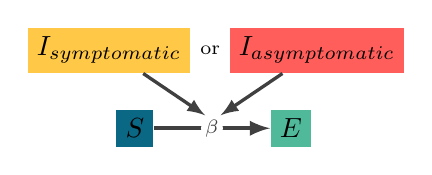
\begin{tikzpicture}[scale=0.66]
    \node at (0.5, 0) (S) [shape=rectangle, fill=S] {$S$};
    \node at (3.5, 0) (E) [shape=rectangle, fill=E] {$E$};
    \node at (0, 1.5) (Is) [shape=rectangle, fill=Is] {$I_{symptomatic}$};
    \node at (1.95, 1.5) (or) [] {\scriptsize or};
    \node at (4, 1.5) (Ia) [shape=rectangle, fill=Ia] {$I_{asymptomatic}$};

    \Edge[Direct, label=$\beta$](S.east)(E.west)

    \path[->, draw, very thick, color=black!75] (Is) -- (1.85,.25);
    \path[->, draw, very thick, color=black!75] (Ia) -- (2.15,.25);
  \end{tikzpicture}
\end{document}
